\section{The Large Hadron Collider and the CMS Detector}

\emph{%
This section covers the Large Hadron Collider and the CMS detector.
% 
}


\subsection{The Large Hadron Collider}

The Large Hadron Collider at CERN is the largest particle accelerator with the highest center-of-mass energy to date.
% 
It is the final stage in a series of accelerators which are part of the CERN accelerator complex, which is illustrated in Fig.~\ref{fig:cernacceleratorcomplex}.
% 
The LHC is built partially in Switzerland and in France, and it is located about 100\unit{m} underground.
% 
Its design corresponds to a \textit{storage ring}, in which particles are kept in a circular trajectory for an extended period of time using powerful superconducting magnets.
% 
The achievable center-of-mass energy for proton-proton collisions, the primary research mode for the LHC, depends on the magnetic field strength of these 1232 bending magnets (about 8.3\unit{T}~\cite{lhc}) and the radius of the ring (about 27\unit{km}).
% 
The latest data from the LHC, including the data used in this thesis, was collected at $\sqrt{s}=13\TeV$.
% 
The LHC employs 16 radiofrequency (RF) cavities in order to create tight particle bunches and to accelerate particles from the insertion energy of about 450\GeV to 6.5\TeV.


\begin{figure}[hbtp]
  \begin{center}
    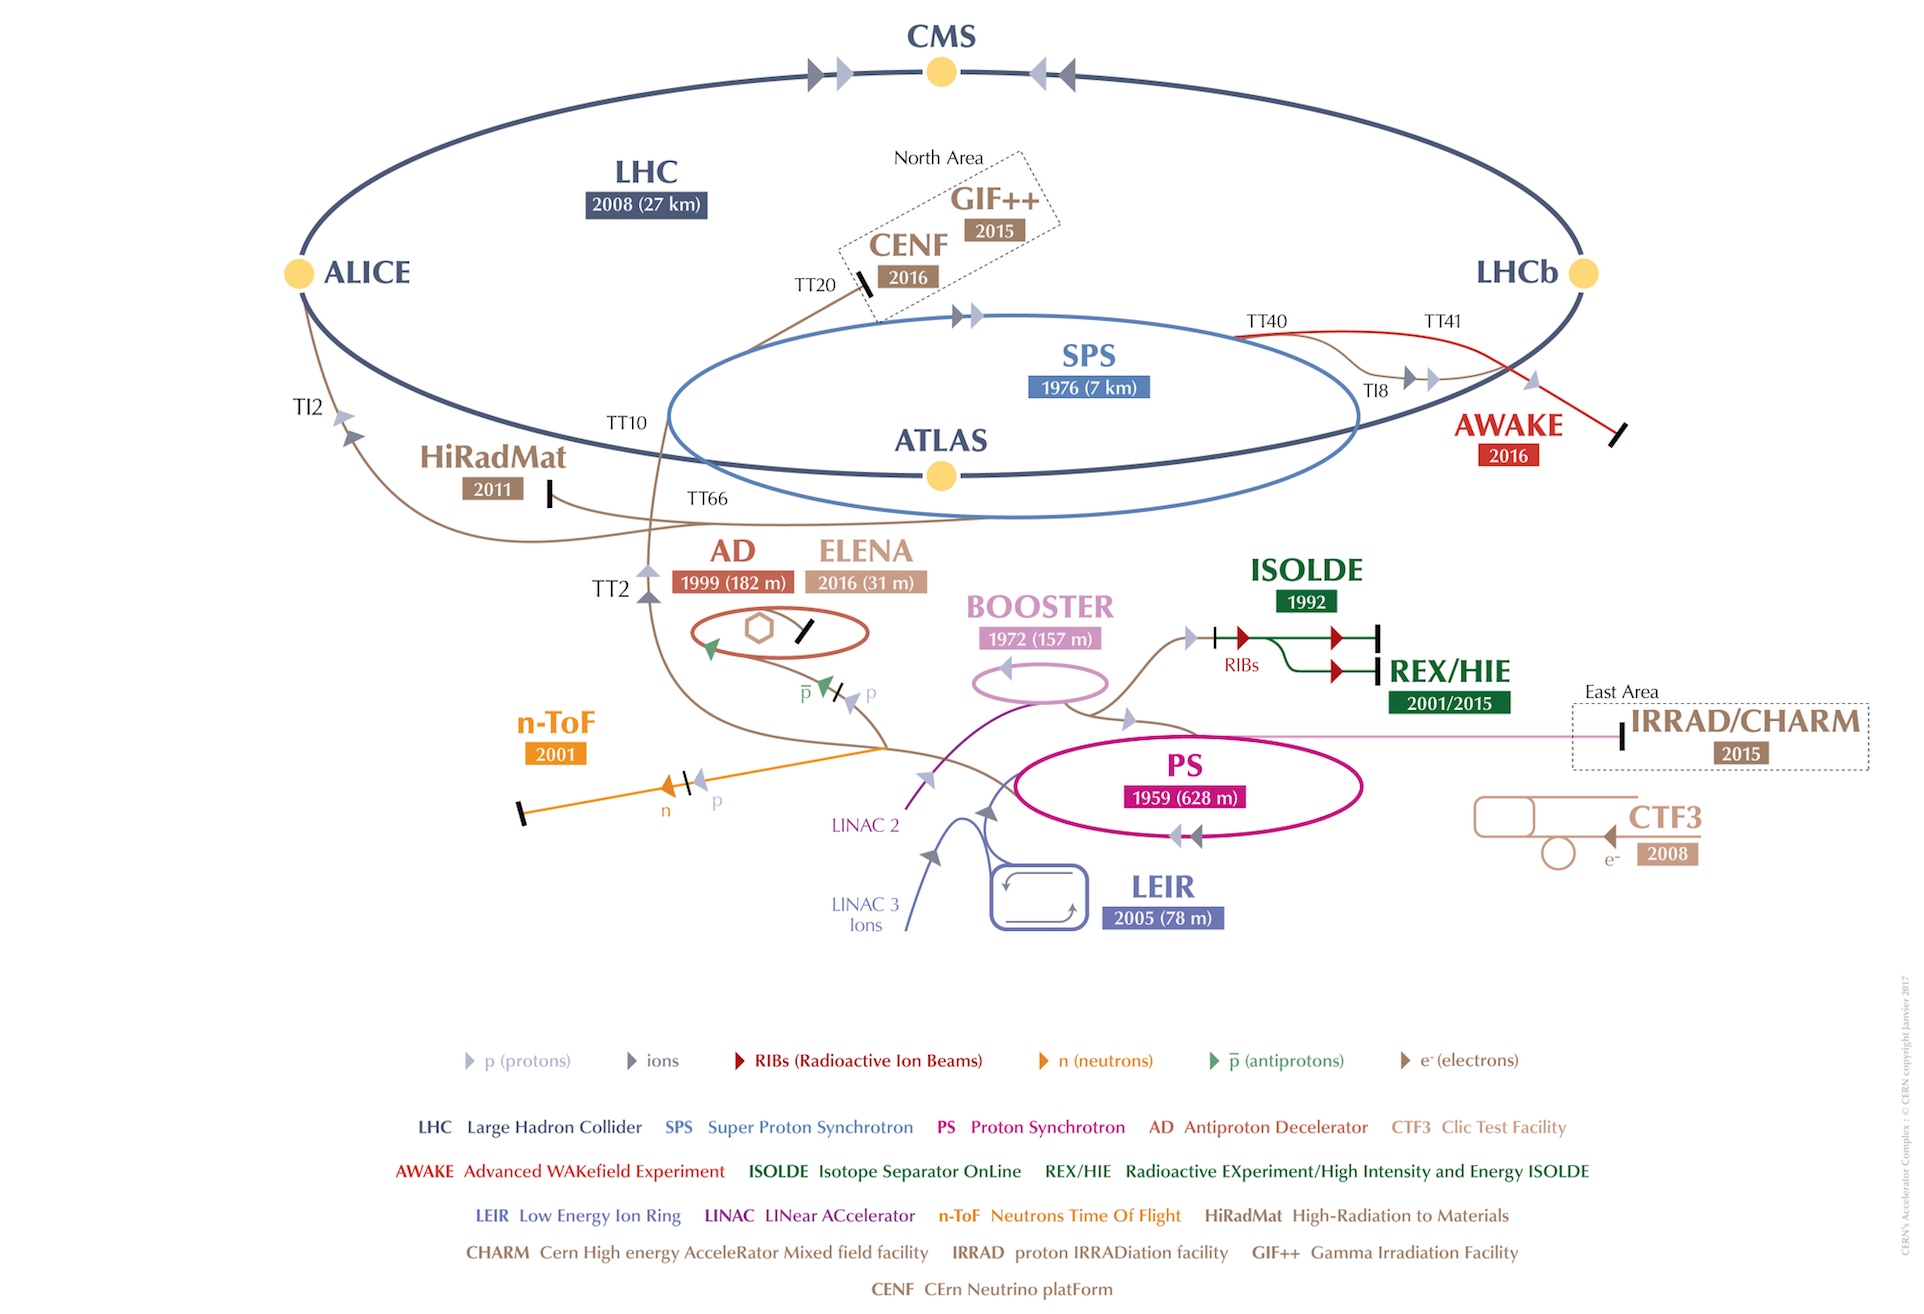
\includegraphics[width=\linewidth]{img/detector/cernacceleratorcomplex_small.png}
    \caption{
        The CERN accelerator complex. Taken from Ref.~\cite{cernacceleratorcomplex}.
        }
    \label{fig:cernacceleratorcomplex}
  \end{center}
\end{figure}


Of the many detectors associated with the CERN accelerator complex, the four most prominent ones are the CMS detector, the ATLAS detector, the LHCb detector, and the ALICE detector.
% 
The CMS and ATLAS detectors are both general-purpose detectors, with a similar physics program meant to yield comparable measurements.
% 
This thesis concerns data from the CMS experiment, and the structure of its detector is treated in more detail in Section~\ref{sec:cmsdetector}.


For any particle physics process, the rate of events $\mathrm{d}R/\mathrm{d}t$ is given by
% 
\begin{linenomath*}
\begin{equation}
\frac{\mathrm{d}R}{\mathrm{d}t} = \sigma \, L_\text{inst}
\,,
\end{equation}
\end{linenomath*}
% 
where $\sigma$ is the cross section of the process and $L_\text{inst}$ is the instantaneous luminosity.
% 
For a given center-of-mass energy, $\sigma$ is a constant; the instantaneous luminosity, however, is a machine quantity that is to be optimized in the design of an accelerator.
% 
For two colliding beams containing an equal number of particles $N$ that are Gaussian-distributed in the plane perpendicular to the direction of motion with a beam width $\sigma_\text{beam}$, the instantaneous luminosity is given by~\cite{griffiths}
% 
\begin{linenomath*}
\begin{equation}
L_\text{inst} =
\frac{
    N^2 f N_b 
    }{
    4 \pi \sigma_\text{beam}^2
    }
\,,
\end{equation}
\end{linenomath*}
% 
where $f$ is the revolution frequency and $N_b$ is the number of bunches.
% 
The \textit{integrated luminosity} $L$ is given by the integral of the instantaneous luminosity over time and is typically expressed in units of \fbinv.
% 
It is the typical quantity employed for indicating the size of a collection of data.


At the time of writing, the LHC has just finished its second data-taking run, colloquially referred to as `Run 2'.
% 
Combined with the first data-taking run, the LHC has delivered almost 200\fbinv, and is expected to deliver around 300\fbinv by the end of the third data-taking run.
% 
The evolution of the delivered luminosity and the collected luminosity by the CMS detector is shown in Fig.~\ref{fig:cmslumi}.

\begin{figure}[hbtp]
  \begin{center}
    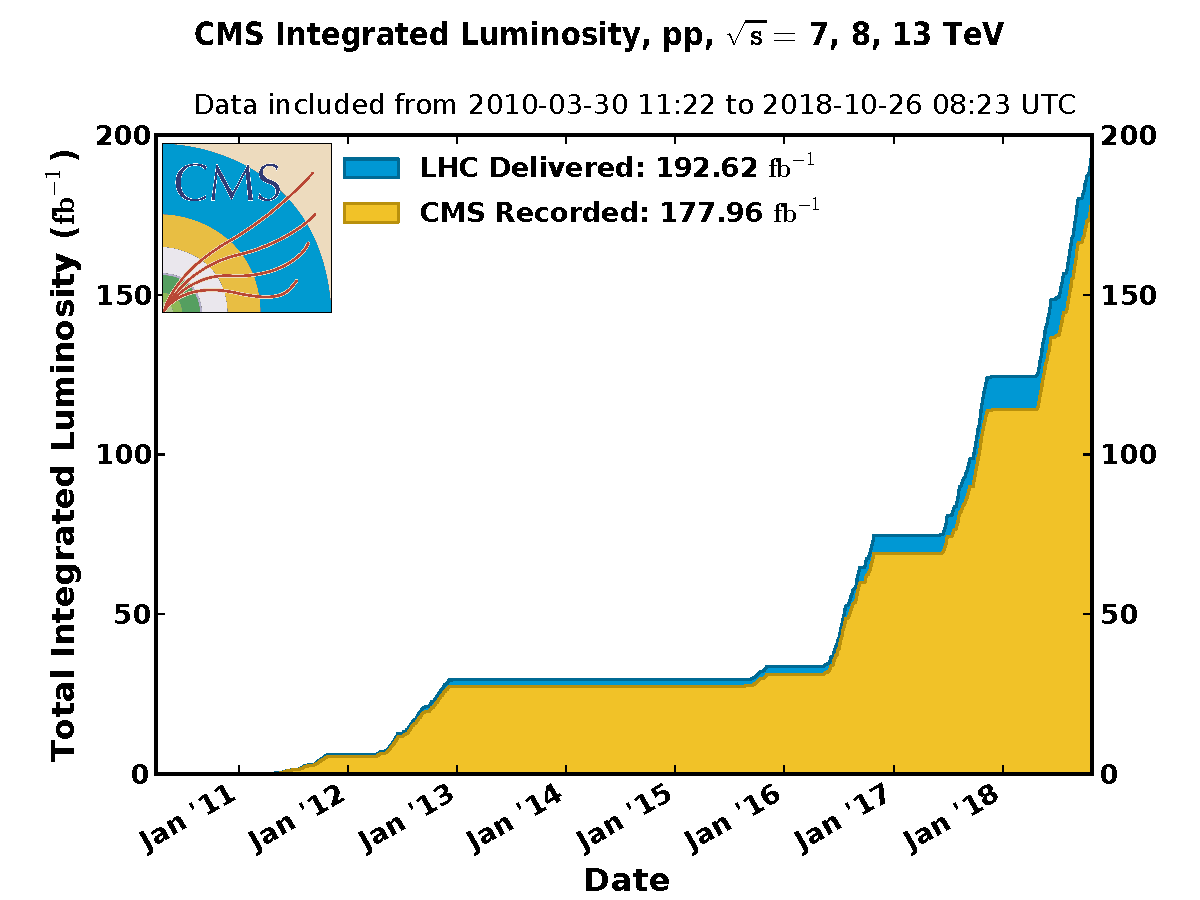
\includegraphics[width=0.7\linewidth]{img/detector/cmslumi.pdf}
    \caption{
        Cumulative delivered and recorded luminosity at the CMS detector versus time for 2010-2012 and 2015-2018.
        % 
        Only proton-proton collision data is taken into account.
        % 
        Taken from Ref.~\cite{cmslumi}.
        }
    \label{fig:cmslumi}
  \end{center}
\end{figure}


\subsection{The CMS detector}
\label{sec:cmsdetector}

As a general-purpose detector, the CMS detector was designed to be able to detect most SM particles over a large range of energy scales.
% 
The cylindrical shape, with the beam axis at its center, provides a nearly complete solid angle coverage, up to a pseudo-rapidity of $\eta \leq 3.0$.
% 
The components of the detector are illustrated in Fig.~\ref{fig:cmsgeometry}; starting from the beam axis, the first detector is the silicon tracker, followed by the electromagnetic calorimeter (ECAL), and the hadron calorimeter (HCAL).
% 
These detectors are enclosed in the superconducting solenoid magnet, which delivers a magnetic field strength of 3.8\unit{T}, is cooled with liquid helium, and is the largest superconducting solenoid to date.
% 
With its 14000 tonnes and its length of 28.7\unit{m}, `Compact Muon Solenoid' seems to be a misnomer at first glance, but for the range of detector applications it provides, the CMS detector can in fact be considered relatively compact.
% 
Of the stable SM particles listed in Section~\ref{sec:sm}, the CMS detector detects electrons, photons, stable hadrons, and muons; the typical trajectories of these particles are illustrated in Fig.~\ref{fig:cmsslice}.
% 
A full description of the CMS detector can be found in Ref.~\cite{Chatrchyan:2008zzk}.


\begin{figure}[hbtp]
  \begin{center}
    \includegraphics[width=\linewidth]{img/detector/cmsgeometry.pdf}
    \caption{
        A 3-dimensional view of the CMS detector with a cut-out section.
        % 
        Taken from Ref.~\cite{Sakuma:2013jqa}.
        }
    \label{fig:cmsgeometry}
  \end{center}
\end{figure}


\begin{figure}[hbtp]
  \begin{center}
    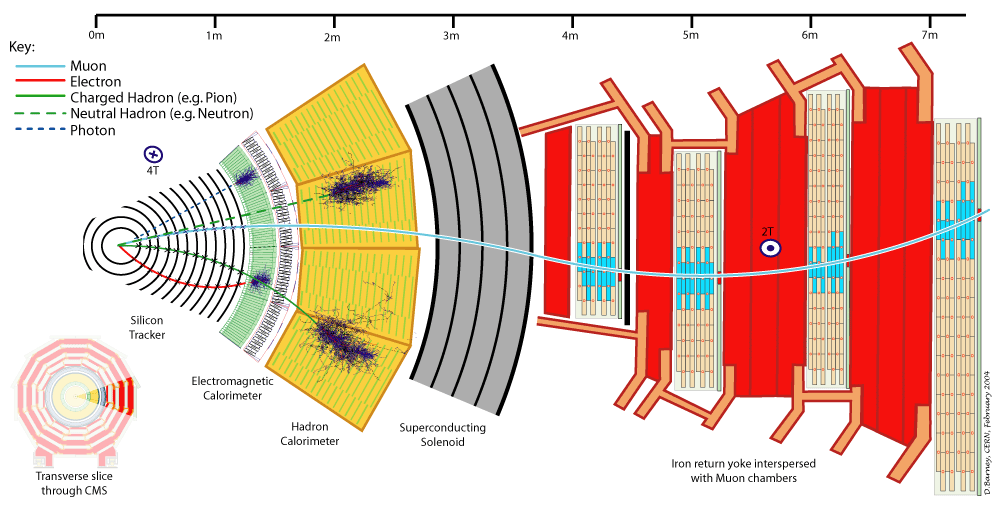
\includegraphics[width=\linewidth]{img/detector/cmsslice.png}
    \caption{
        A transverse slice of the CMS detector.
        % 
        Taken from Ref.~\cite{cmsslice}.
        }
    \label{fig:cmsslice}
  \end{center}
\end{figure}


\subsubsection{The inner tracking system}

The inner tracking system, consisting of a pixel detector surrounded by a silicon strips detector, measures the trajectories of charged particles and reconstructs secondary vertices.
% 
It is designed once again designed cylindrically, with a length of 5.8\unit{m} and a diameter of 2.5\unit{m}, and is able to perform measurements up to $\abs{\eta} \leq 2.5$.
% 
As high radiation levels are part of the operating environment, the tracker is designed to be radiation hard.
%
An important design parameter of the inner tracker is the material budget, which directly affects the achievable resolution of the other subdetector systems; the complete inner tracker corresponds to 0.4 radiation lengths in the central region, and increases up to almost 2 radiation lengths in the forward regions~\cite{Chatrchyan:2008zzk}.
% 
The trajectory is precisely measured with 11 to 17 trajectory points, which requires 66 million pixels and 91 million strips in the pixel and strips detectors, respectively.
% 
The inner tracker is the most important subsystem for low-energy particles; for single muons up to 100\GeV and $\abs{\eta} \leq 1.6$, the \pt resolution is around 1-2\%.


\subsubsection{The electromagnetic calorimeter}

The electromagnetic calorimeter, starting at an inner radius of 1.3\unit{m}, is responsible for the energy measurement of charged particles, and is in particular important for the high-precision measurement of the energy of photons and electrons.
% 
It consists of 61200 lead-tungstate crystals in the barrel region, which have a length of 230\unit{mm} and correspond to 25.8 radiation lengths.
% 
Lead-tungstate crystals have a short scintillation time, are optically clear, and relatively radiation hard.
% 
The barrel region is organized into 36 \textit{supermodules}, each of which consists of 4 \textit{modules}.
% 
The modules further removed from the interaction point have their crystals tilted, so that the front face of the crystal is aimed at the interaction point.
% 
The barrel covers the measurements up to $\abs{\eta} \leq 1.479$.
% 
The forward regions are covered by two endcaps approximately 3\unit{m} from the interaction point in the longitudinal direction, which extend up to $\abs{\eta} \leq 3.0$ and consist of 7324 identical crystals each.
% 
Also these crystals are slanted so that the small front face of the crystal points to the interaction point.
% 
The endcaps are prefaced by the 20\unit{cm} thick \textit{preshower}, whose primary purpose is the enhanced identification of neutral pions in the forward region.
% 
The preshower is a sampling calorimeter that consists of two layers, each containing a lead plate (which initiates electromagnetic showers) and a silicon strip sensor (which measures the deposited energy and the transverse shower profile).


The energy resolution of photons, $\sigma_E$, is of utmost importance for the identification of Higgs bosons in the $\hgg$ decay channel.
% 
Given a photon energy $E$, the relative resolution can be parametrized as~\cite{CMS:1997ysd}
% 
\begin{linenomath}
\begin{equation}
\left( \frac{\sigma_E}{E} \right)^2 =
    \frac{\sigma_\text{noise}^2}{E^2}
    + \frac{\sigma_\text{stoch}^2}{E}
    + c^2
\,,
\end{equation}
\end{linenomath}
% 
where $\sigma_\text{noise}$ is the noise contribution (including e.g. electronic noise and noise related to pileup), $\sigma_\text{stoch}$ is the (irreducible) stochastic contribution, and $c$ is a constant term.
% 
The direct energy measurement performed in ECAL, called the \textit{raw energy} $E_\text{raw}$, is corrected based on other measurable quantities, such as the location of the particle in the detector and the shape of the shower.
% 
This correction is called the \textit{energy regression}, which is recomputed for every dataset recorded by the CMS detector.
% 
More details on the photon and electron energy regressions for the 2016 dataset can be found in Appendix~\ref{ENERGYREGRESSION}.
% 
Under the optimized operating conditions in the CMS detector, the energy resolution for electrons and photons with $10 < E < 2000\GeV$ is about 1\%.
% 
At approximately $E > 2000$\GeV, the lead-tungstate crystal read-out becomes \textit{saturated}, meaning the measured raw energy is often simply the maximum allowed value of the analog-to-digital converter.
% 
In this case the raw energy is a poor estimate of the true energy, and the shower shape becomes the leading determinant for the corrected energy.
% 
For the very-high-energy regime, up to about $6500$\GeV, the energy resolution is at the order of a few percent.



\subsubsection{The hadron calorimeter}

The hadron calorimeter, called HCAL, is located between ECAL and the superconducting solenoid, starting at an inner radius of $1.77$\unit{m} and ending at an outer radius of $2.95$\unit{m}.
% 
Its primary purpose, as its name suggests, is the accurate energy measurement of hadrons, in particular neutral ones that leave no traces in the inner tracking and ECAL subsystems.
% 
Like the previously treated subdetector systems, it is designed cylindrically with a barrel region extending up to $\abs{\eta} < 1.3$ and two endcaps extending up to $\abs{\eta} < 3.0$.
% 
As the combined stopping power of the ECAL and HCAL barrel regions is still insufficient for some high energy particles, the HCAL is extended outside the superconducting solenoid by the HCAL Outer Calorimeter, which measures the shower energy deposited after the HCAL barrel.
% 
HCAL is a sampling calorimeter, composed of brass absorber plates and plastic scintillators, which are optimized for longterm stability and radiation hardness.


\subsubsection{The muon system}

The CMS muon system is responsible for the identification and measurement of muons, and simultaneously serves as an important part of the trigger system.
% 
Muons can be considered stable particles in the context of particle detection at CMS, and unlike most particles they are not stopped by the ECAL and HCAL subdetector systems.
% 
Their detection relies on measurements in the inner tracker and the muon system, which is placed outside the superconducting solenoid and interleaved with the iron flux return yoke plates.
% 
The muon system comprises four layers of muon detection, which measure the curvature of the muon track in order to determine its energy---the principle is illustrated in Fig.~\ref{fig:cmsslice}, where the light blue hits in the outer layers trace the muon trajectory.
% 
The barrel region of the muon system employs drift tubes, arranged in such a way to accurately measure the muon coordinates while preventing dead spots in the efficiency.
% 
In the endcaps the neutron-induced background and the muon rate are much higher and the magnetic field is non-uniform; here cathode strip chambers are employed, which operate more reliably under these circumstances.
% 
In addition, a redundant trigger system was put in place consisting of cathode strip chambers, in both the barrel and endcap regions.


\subsubsection{The trigger and data acquisition systems}

At the peak of the LHC instantaneous luminosity, bunch crossings take place in the CMS detector at a rate of about 40\unit{MHz}, yielding at the order of a billion proton-proton interactions per second.
% 
The size of the full, uncompressed data collected from a single bunch crossing, typically called an \textit{event}, is over a megabyte.
% 
The rate at which data is accumulated far surpasses the storage capabilities and the processing rate available to the CMS experiment; instead, only a fraction of the detected events is kept, based on signatures in the events that indicate potentially interesting physics.
% 
The very first stage of event selection at CMS is the \textit{Level-1 (L1) trigger}, whose implementation relies mostly on programmable hardware.
% 
It is designed to accept events at the rate of about 100\unit{kHz}, using an algorithm based on hits in the muon system and in the calorimeter subdetectors.
% 
While the decision to accept or reject is made, which may take at most 3.2\unit{$\mu$s}, the full event is kept in buffers of the front-end electronics.


When an event is accepted, the full event is passed to the \textit{High Level Trigger (HLT)}~\cite{Adam:2005zf}, which is implemented as a software running on a dedicated computer cluster.
% 
Its decision-making time is longer than the L1 trigger and its algorithms more involved; it can reconstruct final-state objects (at a limited precision) and accept events based on current analysis needs.
% 
Events are ran in parallel through several \textit{trigger paths}, each of which can accept the event (even if other paths rejected the event).
% 
The HLT reduces the event rate to about 1\unit{kHz}, at which point the event is stored on a central storage server at CERN, and passed along to the Worldwide LHC Computing Grid for reconstruction.



\subsubsection{Particle-flow reconstruction in the CMS detector}

The detection capabilities per subdetector
% , outlined in Section~\ref{sec:cmsdetector},
are generally combined into a single picture of a particle physics event, which is then used for further physics analysis.
% 
For example, while the muon system shines in terms of muon identification and momentum measurement, its performance can be increased be including measurements from the inner tracker system.
% 
This holistic approach of including as much useful subdetector information as possible into the particle reconstruction algorithm is, within the CMS detector, called \textit{particle-flow (PF) reconstruction}~\cite{Sirunyan:2017ulk}.
% 
Here a summary of the particle-flow procedure is treated; a full description can be found in Ref.~\cite{Sirunyan:2017ulk}.
% 
The primitive building blocks, called the \textit{PF elements}, are the \textit{tracks} and \textit{hits} in the inner tracker, ECAL, HCAL, and the muon system, and the \textit{vertices}.
% 
The PF elements are \textit{linked} into associated sets of elements called \textit{PF blocks}, from which particles are finally reconstructed.
% 
Per PF block, the algorithm first identifies and reconstructs muons, and subsequently removes the elements associated with the muons from the block.
% 
Secondly, the electrons are identified and reconstructed, aiming to take into account photons from bremsstrahlung into account as well.
% 
Isolated photons with high energy are identified and reconstructed simultaneously, leaving hadrons from jet fragmentation and hadronization.
% 
Hadrons are typically detected either as charged hadrons (with a track, and hits in the calorimeters), neutral hadrons, nonisolated photons (usually stemming from the $\pi^0$ decay to two photons).
% 
After reconstruction of all particles, a post-processing step is applied, correcting for, among other things, cosmic muons, muons decaying inside the detector, and misidentified muons due to punch-through of hadrons through HCAL.


\subsection{The Worldwide LHC Computing Grid}

The computing resources available at CERN are insufficient to reconstruct and analyze all the data that is produced at the LHC experiments.
% 
Rather than localizing all computing resources at CERN, instead the resources are scattered all over the globe and are organized in a distributed computing infrastructure, the \textit{Worldwide LHC Computing Grid} (WLCG), following the principles described in Ref.~\cite{thegrid}.
% 
The WLCG provides over 10000 grid users nearly real-time access to its data storage and computing resources~\cite{wlcgwebsite}; users of the grid only specify their computing needs, and the grid dispenses the computing load to its available resources.
% 
The grid is organized into four \textit{tiers} with varying responsibilities, here described in the context of the CMS experiment~\cite{Bayatyan:838359,CMS:2005aa}:
% 
\begin{itemize}
\item \textbf{Tier 0:} The first tier takes all raw, uncompressed data, called the \emph{RAW datatier}, from the CMS detector for a first pass of the event reconstruction, and archives the RAW data to tape storage.
% 
The partially-reconstructed data is then sent to the Tier-1 sites for further processing.
% 
The Tier-0 resources are also used for the reprocessing of data when no new data is taken by the detectors (i.e. during downtimes of the LHC).
% 
There are two Tier-0 sites; the first, primary site is located at CERN, and the second is located at the Wigner Research Centre for Physics in Budapest, Hungary.
% 
These two physical sites, separated by 1200\unit{km}, are connected via three dedicated 100\unit{Gbit/s} data links.
% 
Developments are ongoing with the enabling of Tier-0 workflows on other computing sites, such as the CMS Tier-2 site at CSCS in Lugano, Switzerland.
% 
\item \textbf{Tier 1:} The main responsibility of the Tier-1 facilities is to provide the permanent storage of all active CMS datasets, and to provide fast access to any of its datasets worldwide to any authorized user.
% 
The Tier-1 computing resources are used for reconstruction and other low-level data processing; physics analysis workflows are not performed at the Tier-1 level.
% 
At the time of writing, there are 13 active Tier-1 sites (not just dedicated to CMS), listed in Fig.~\ref{fig:wlcg}
% 
\item \textbf{Tier 2:} The Tier-2 facilities provide limited storage, relying mostly on the Tier-1 sites for very large datasets.
% 
The Tier-2 computing resources are used primarily for event simulation and reconstruction workflows from CMS, but at this tier also private data-analysis workflows and private storage is available to grid users.
% 
At the time of writing, there about 160 active Tier-2 sites for all experiments at the LHC.
% 
\item \textbf{Tier 3:} The final tier consists of small, private computing clusters.
% 
There are only few formal requirements in order for a site to be considered a Tier-3 site, and the other tiers of the grid do not rely on the functioning of Tier-3 sites.
% 
This last tier is typically fully dedicated to research groups, and has not just data-analysis workflows enabled, but also custom distributed-computing setups.
% 
It is usually also the access point for users to the grid, providing tools for the interaction with datasets stored on the Tier-1 and 2 levels and tools to submit analysis jobs to the Tier-2 computing resources.
% 
The analysis carried out in this thesis has been performed exclusively on the Tier-3 site at the Paul Scherrer Institut in Villigen, Switzerland.
% 
\end{itemize}


\begin{figure}[hbtp]
  \begin{center}
    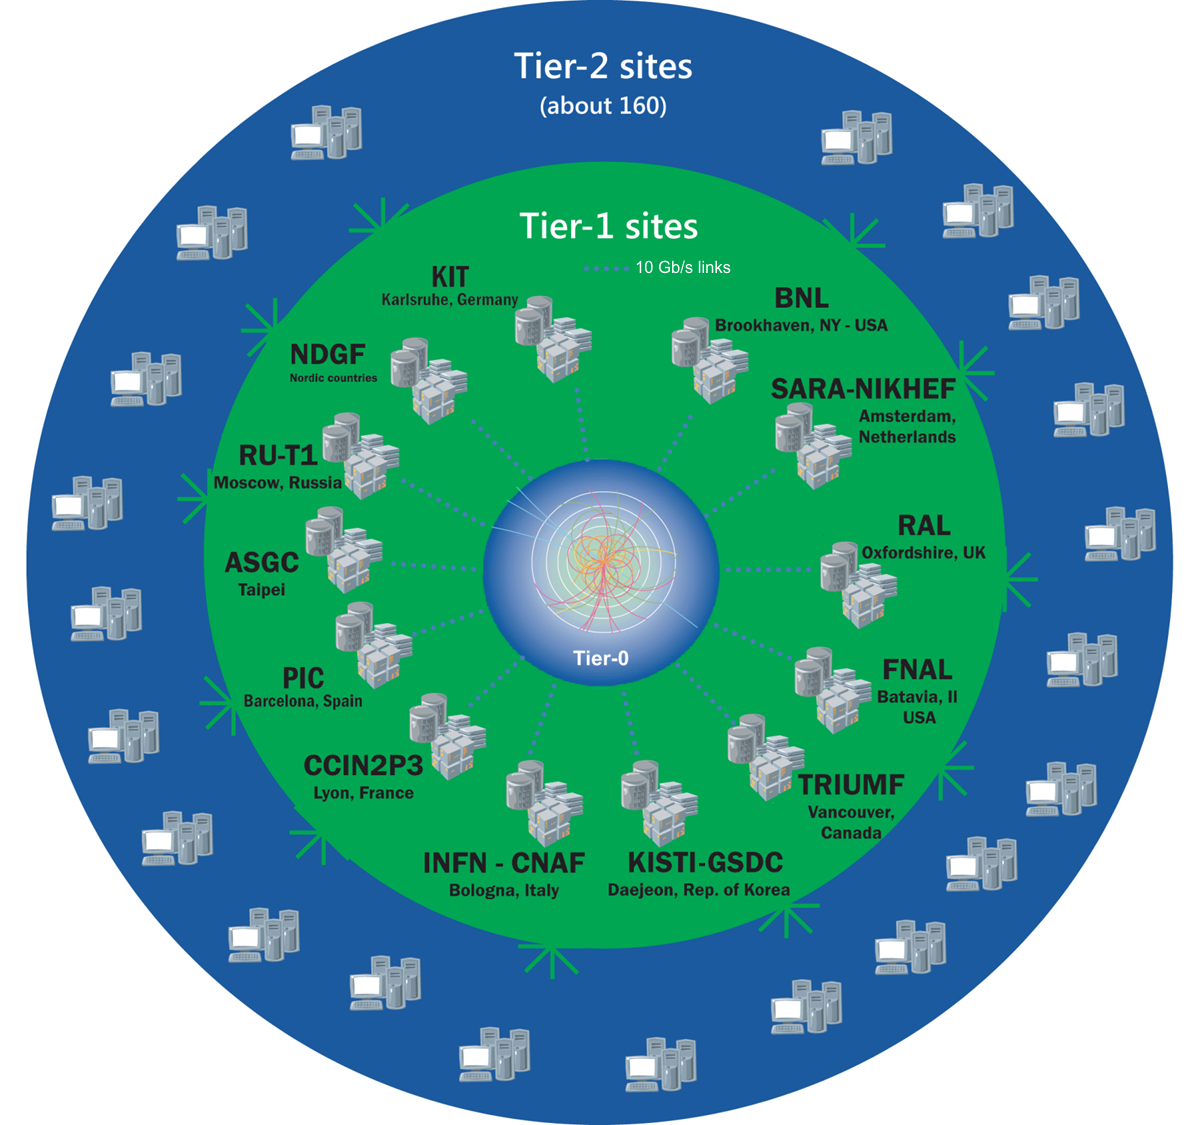
\includegraphics[width=0.7\linewidth]{img/detector/wlcg.png}
    \caption{
        Tiers of the WLCG. Taken from Ref.~\cite{wlcgwebsite}.
        }
    \label{fig:wlcg}
  \end{center}
\end{figure}

